\documentclass[10pt]{article}

\usepackage[T1]{fontenc}
\usepackage[margin=0.82in]{geometry}
\usepackage{amsmath}
\usepackage{booktabs}
\usepackage{graphicx}
\usepackage[protrusion=true,expansion=false]{microtype}
\usepackage{xcolor}
\usepackage{hyperref}
\usepackage{url}

\graphicspath{{figures/}}
\hypersetup{colorlinks=true,linkcolor=blue!55!black,urlcolor=blue!55!black}

\title{AI Collectives in gem5 Garnet\\
\large Multicast, Bypass Links, and Real-H100 Trace Replay}
\author{Lab 4 Project Team}
\date{August 7, 2026}

\begin{document}
\maketitle

\begin{abstract}
This report evaluates three related interconnection mechanisms implemented in
gem5 Garnet: router-level tree multicast, express-link bypass routing, and
trace-driven broadcast/all-reduce traffic.  The multicast regression passes
208 paired correctness cases and its 162-case performance matrix reduces
internal-link flit traffic by 39.2\% on average with a 3.59$\times$ median
completion-latency speedup, while retaining ten negative throughput cases.
The bypass study shows that optimistic shortcut latency is an upper bound:
distance-scaled links can regress, and a tree-sharing-aware policy must reject
shortcuts that destroy multicast reuse.  Finally, an executed eight-H100 NCCL
microbenchmark drives 30 broadcast requests (6,720 flits) and 6,720 scalar
all-reduce lanes (53,760 rank contributions) to exact completion on paired
Mesh and Bypass topologies.  These are mechanism and scaled-trace results, not
measurements of a complete model, NVLink/NVSwitch, or vector reduction
hardware.
\end{abstract}

\section{Scope and Research Question}

The multicast portion of Topic 3 asks whether one source can deliver a packet
to multiple destinations with one logical injection instead of transmitting
one complete copy per destination.  We answer the following question:

\begin{quote}
For the same source, destination set, payload, request schedule, and network
configuration, how does router-level tree replication compare with source-side
replicated unicast in traffic, completion latency, and throughput?
\end{quote}

This distinction is important.  A broadcast that always visits every router
does not implement arbitrary multicast, and an all-reduce broadcast is not a
fair multicast baseline.  Our implementation carries a 64-bit destination
bitmap, prunes unused branches, and generates a local copy only when the local
router belongs to the destination set.  The current bitmap limits one
multicast domain to at most 64 routers.

The bypass portion asks whether added long-range links can reduce ordinary
Mesh traversal without ignoring wire length, radix, buffering, or multicast
tree sharing.  Topic 4 asks whether a collective trace captured on real GPUs
can deterministically drive the same Garnet mechanisms with auditable scaling
and exact completion checks.  We report these questions separately because a
correct mechanism, a synthetic performance result, and a trace replay provide
different levels of evidence.

\section{Architecture and Baseline}

\subsection{Replicated-unicast baseline}

For a logical destination set of size $N$, the source Network Interface (NI)
creates one normal deterministic-XY packet for every remote destination.  A
local destination completes locally and creates no internal-link traversal.
Each physical packet uses the standard Garnet input buffering, route
computation, VC allocation, switch allocation, and credit flow control.  All
copies retain the same logical multicast identifier and round identifier.

\subsection{Tree multicast}

The source injects one physical packet.  Its head flit carries the destination
bitmap and establishes persistent output-branch state at each router.  Body
and tail flits use the same branch set.  A router sends a flit only when all
selected branches have the required VC or credit, preventing a partially
replicated flit from being dropped or duplicated.  The tail releases branch
VCs and per-packet state.  This atomic-fanout behavior is conservative: it
preserves correctness under backpressure but can make a fast branch wait for
a congested branch.

\subsection{Common completion contract}

A logical request completes only when every expected destination has received
exactly one complete packet with the correct identifier and payload.  Missing,
duplicate, unexpected, or wrong-round delivery is fatal.  Reaching the
simulation tick limit is not accepted as successful completion.

\section{Experimental Method}

Table~\ref{tab:matrix} summarizes the performance matrix generated by
\texttt{run\_multicast\_performance.py}.  Every row is run once with replicated
unicast and once with tree multicast using identical parameters.  Warmup and
cooldown requests are excluded from measured latency and throughput.

\begin{table}[ht]
\centering
\caption{Current paired performance matrix.}
\label{tab:matrix}
\begin{tabular}{ll}
\toprule
Parameter & Values \\
\midrule
Topology & 4$\times$4 Mesh, deterministic XY tree \\
Source router & 5 \\
Destination count & 4, 8, 16 \\
Packet size & 1, 4, 16 flits \\
Offered request probability & 0.1, 0.5, 1.0 \\
Background unicast rate & 0.0, 0.1 \\
Random seeds & 1, 7, 17 \\
Phases & 20 warmup, 100 measured, 20 cooldown requests \\
Maximum outstanding requests & 8 \\
Paired cases / raw runs & 162 / 324 \\
\bottomrule
\end{tabular}
\end{table}

The derived metrics are
\begin{align*}
S_L &= L_{\mathrm{naive}} / L_{\mathrm{tree}}, \\
R_T &= 1 - F_{\mathrm{tree}} / F_{\mathrm{naive}}, \\
I_Q &= Q_{\mathrm{tree}} / Q_{\mathrm{naive}} - 1,
\end{align*}
where $L$ is logical-request completion latency, $F$ is measured internal-link
flit traversal, and $Q$ is completed logical multicasts per cycle.  Absolute
values are retained in the released CSV and JSON files.

\section{Correctness Evidence}

The current correctness command reruns both modes for 26 source/destination
configurations and four packet sizes, producing 208 paired cases.  It includes
all 15 nonempty destination masks in a 2$\times$2 network, source-included and
source-excluded cases, local-only delivery, row/column groups, sparse groups,
and random groups on 3$\times$3 and 4$\times$4 meshes.  Packet sizes are 1, 4,
16, and 64 flits.  All 208 cases passed in the audited run on August 7, 2026.

The runner checks the final destination bitmap, completion-driven exit,
logical request count, destination delivery count, source flits,
router-generated flits, physical packet count, and zero reduction merges.  It
therefore checks exact small-topology traffic invariants in addition to
successful termination.

\section{Performance Results}

\subsection{Physical traffic}

Figure~\ref{fig:traffic} shows that traffic reduction grows with multicast
fanout.  The average reduction is 29.1\% for four destinations, 35.3\% for
eight destinations, and 53.1\% for all 16 destinations.  The overall mean is
39.2\%, with a range from 11.1\% to 53.1\%.  Variation at group size four is
caused by the geometry of the randomly selected destination set: destinations
with more overlapping XY paths provide more replication reuse.

\begin{figure}[ht]
\centering
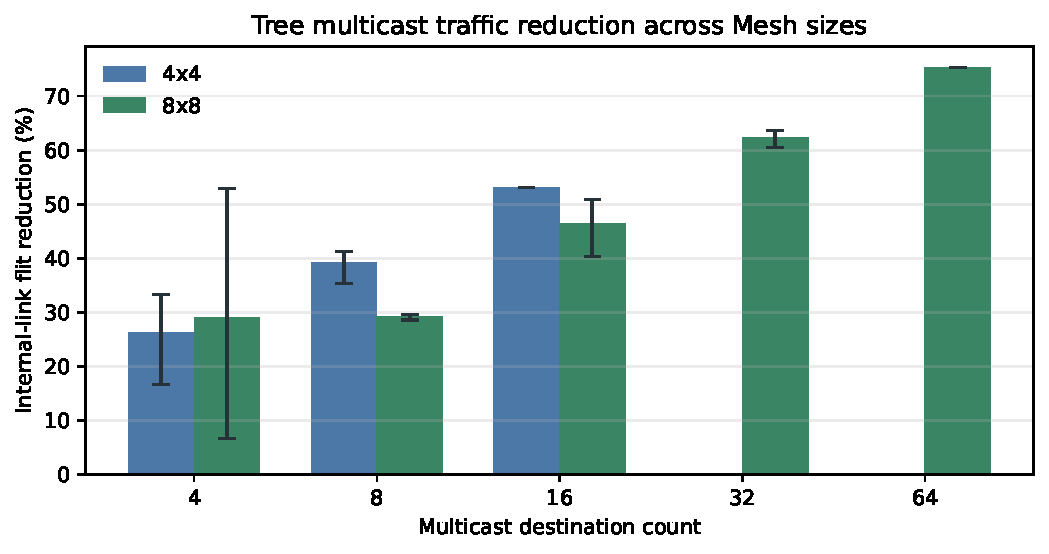
\includegraphics[width=0.82\linewidth]{traffic_reduction_by_group.pdf}
\caption{Mean internal-link flit reduction.  Error bars show the observed
minimum and maximum across paired cases, not a confidence interval.}
\label{fig:traffic}
\end{figure}

\subsection{Completion latency}

Figure~\ref{fig:latency} reports latency speedup grouped by fanout and packet
size.  Every measured paired case has $S_L>1$, with an overall mean of
4.79$\times$, median of 3.59$\times$, and range of 1.20$\times$ to
22.51$\times$.  The increasing benefit with destination count is expected:
replicated unicast serializes or contends among more source-generated copies,
while the tree shares common path prefixes.

The very large maximum for four-flit packets should not be generalized beyond
this matrix.  It combines particular destination placement, bounded
outstanding requests, and source-side replication pressure.  The final study
must retain per-case results instead of reporting only the mean.

\begin{figure}[ht]
\centering
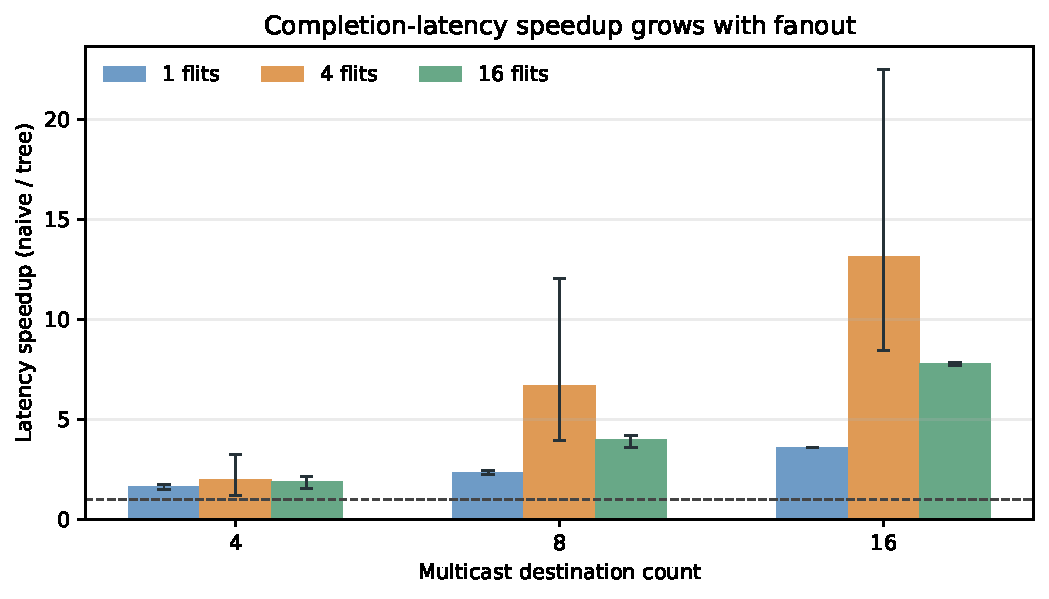
\includegraphics[width=0.92\linewidth]{latency_speedup_by_group.pdf}
\caption{Completion-latency speedup.  Bars are arithmetic means and error
bars span the observed minimum and maximum.  The dashed line is break-even.}
\label{fig:latency}
\end{figure}

\subsection{Throughput and contention}

Figure~\ref{fig:heatmap} shows the mean throughput change by fanout and packet
size.  Full-group multicast benefits strongly because it removes many
source-generated copies.  Small-group, long-packet traffic benefits much less:
the four-destination, 16-flit cell improves by only 1.5\% on average.

\begin{figure}[ht]
\centering
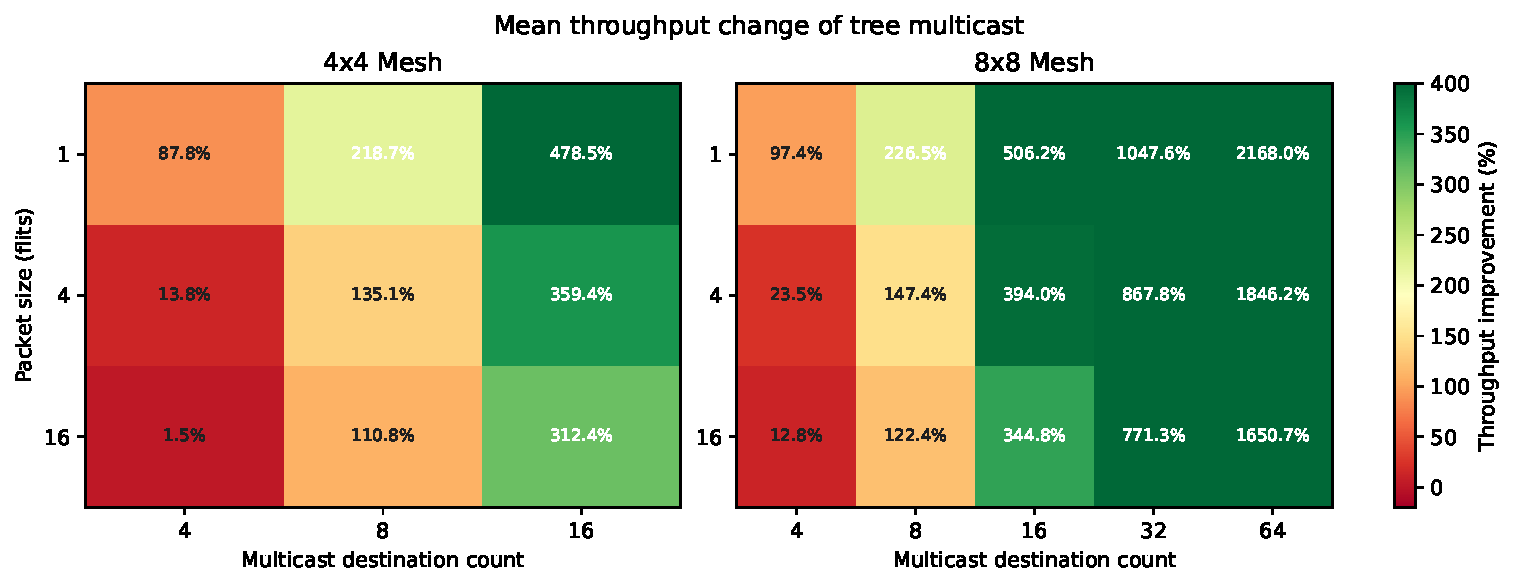
\includegraphics[width=0.78\linewidth]{throughput_improvement_heatmap.pdf}
\caption{Mean throughput improvement over all offered-load, background, and
seed settings for each fanout/packet-size pair.}
\label{fig:heatmap}
\end{figure}

Figure~\ref{fig:load} gives absolute throughput for full-group multicast with
no background traffic.  The 0.5 and 1.0 offered-probability points frequently
coincide.  With at most eight outstanding requests, these points exercise a
bounded-outstanding regime rather than providing a finely resolved saturation
curve.  Additional offered-load points and accepted-load reporting are needed
for the final saturation analysis.

\begin{figure}[ht]
\centering
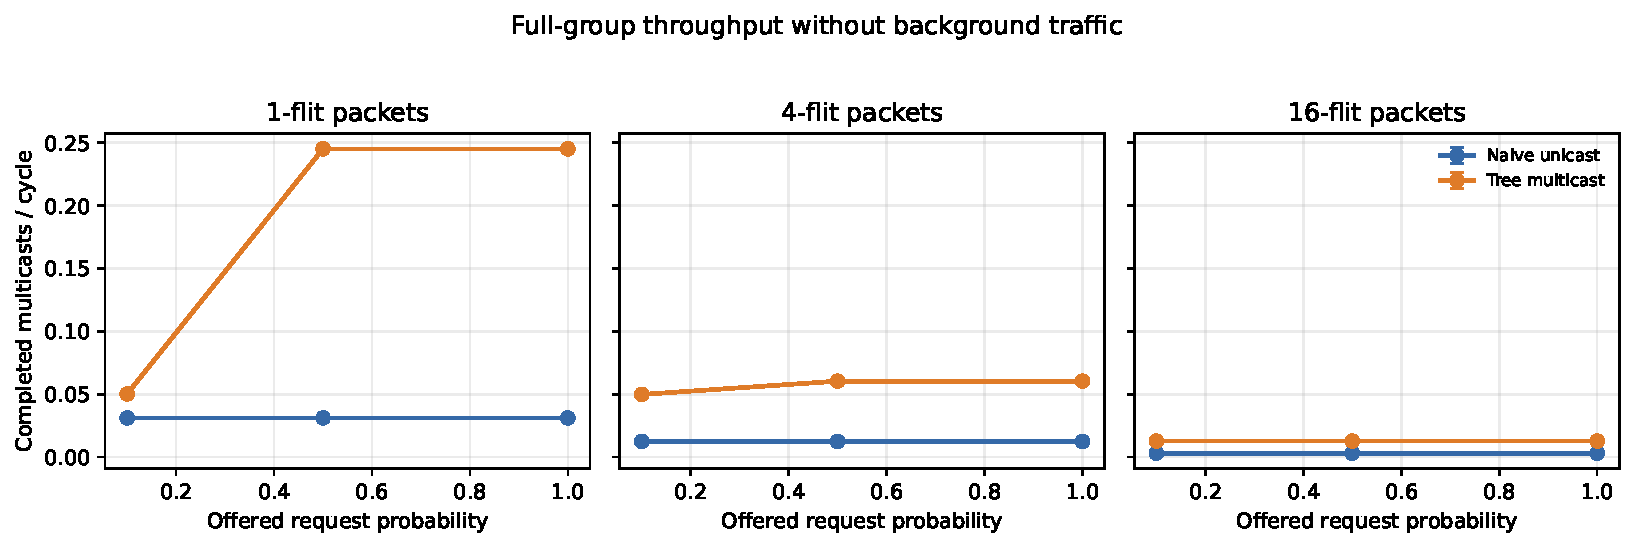
\includegraphics[width=\linewidth]{throughput_vs_offered_load.pdf}
\caption{Full-group throughput.  Points are means over three seeds; error bars
show one standard deviation.}
\label{fig:load}
\end{figure}

The overall mean throughput change is +190.9\% and the median is +121.7\%, but
the distribution is skewed by high-fanout cases.  As shown in
Figure~\ref{fig:distribution}, 10 of 162 cases (6.2\%) regress.  All regressions
occur for four-destination groups; the worst case is a 16-flit packet with
seed 17, no background traffic, and offered probability 0.5 or 1.0.  It has
33.3\% less link traffic and 1.55$\times$ lower completion latency, yet its
steady-state throughput is 18.2\% lower.  This is consistent with the atomic
fanout policy: reduced traffic does not guarantee that every branch can make
progress independently.

\begin{figure}[ht]
\centering
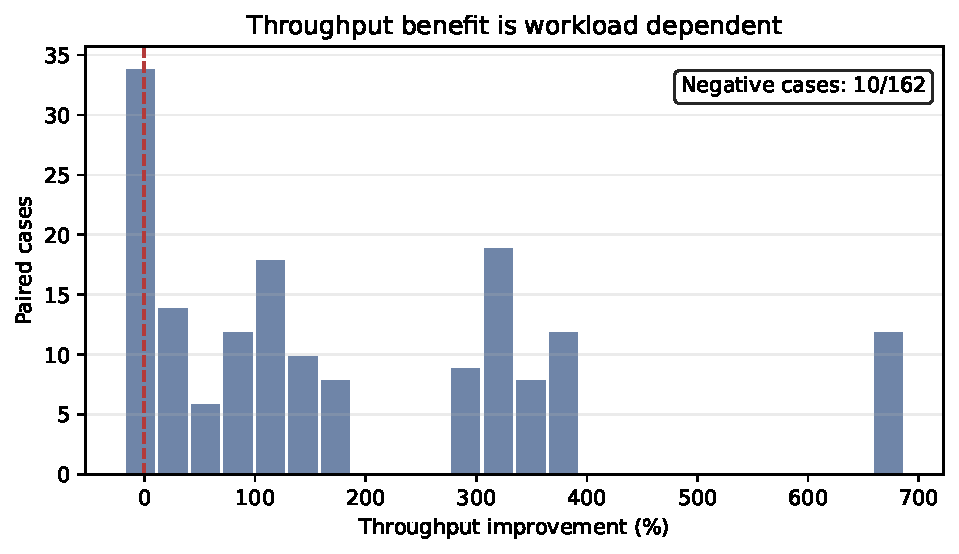
\includegraphics[width=0.82\linewidth]{throughput_improvement_distribution.pdf}
\caption{Distribution of throughput improvement.  The dashed line marks no
change.  Negative cases must remain visible in the final conclusion.}
\label{fig:distribution}
\end{figure}

Tree-mode credit stalls are nonzero in 45 of 162 raw tree runs, with a maximum
of 411 recorded stalls.  This confirms that the performance matrix exercises
backpressure, although it does not replace an explicit low-buffer/one-VC
stress matrix.

\section{Bypass Links and Multicast Interaction}

The bypass extension augments the ordinary Mesh with diagonal or stride
express links.  Each placement is evaluated with an optimistic one-cycle
model and a distance-scaled model whose serialization/latency reflects the
link's Manhattan span.  The G9 matrix contains 7,680 successful gem5 runs,
6,144 paired seed cases, two Mesh sizes, four traffic patterns, four packet
sizes, 16 offered-load points, and three seeds.

\begin{table}[ht]
\centering
\caption{Mean bypass results over the full synthetic matrix.}
\label{tab:bypass}
\begin{tabular}{lrrr}
\toprule
Design & Latency speedup & Throughput change & Traversal change \\
\midrule
Diagonal, distance-scaled & 1.629$\times$ & +6.41\% & $-$2.82\% \\
Diagonal, optimistic & 1.723$\times$ & +10.61\% & $-$7.03\% \\
Stride, distance-scaled & 0.981$\times$ & $-$1.94\% & +15.50\% \\
Stride, optimistic & 1.103$\times$ & +3.68\% & +10.10\% \\
\bottomrule
\end{tabular}
\end{table}

The aggregate table alone is not a hardware claim.  At offered load at most
0.1, diagonal and stride distance-scaled mean latency speedups are only
0.962$\times$ and 0.936$\times$, respectively.  Diagonal placement also adds
9 undirected links, wire-length proxy 18, and maximum Router radix 8 on the
4$\times$4 Mesh; the corresponding 8$\times$8 values are 49, 98, and 8.
Thus fewer Router traversals do not guarantee lower latency after long-wire
and port costs are represented.

G10 explicitly tests multicast interaction in 624 runs.  Replicated unicast
can select express links, but distance-scaled bypass averages 0.965$\times$
latency speedup and becomes worse as packets grow.  Tree multicast preserves
its ordinary XY sharing tree and reports 1.000$\times$ with zero express
flits.  A later directed cost-aware gate proves the joint path is active:
a sparse diagonal-only 2$\times$2 destination completes in 3,500 rather than
4,000 ticks (12.5\% faster), whereas a shared three-destination tree retains
ordinary XY edges.  On the full all-rank broadcast replay the policy also
chooses zero express flits, avoiding the measured 19.4\% forced-bypass
regression.

\section{Real-H100 Trace Replay}

The checked-in source was captured by actually executing a controlled NCCL
collective microbenchmark on eight NVIDIA H100 80GB HBM3 GPUs using CUDA 12.8,
PyTorch 2.8.0+cu128, and NCCL 2.27.3.  It contains 48 events, including 15
measured broadcasts and 15 measured all-reduces at 1, 4, and 16 MiB.  It is
not a complete model or optimizer trace.  Both byte volume and relative event
time are explicitly scaled by 1/1024 for cycle-accurate simulation.

Broadcast events lower to variable-length tree-multicast requests.  All-reduce
events lower differently: the Router reduction datapath accepts one scalar
flit per rank and active lane, so each scaled tensor becomes independent
single-flit lanes.  Every lane performs a real Router-side reduce followed by
tree broadcast; it is not decomposed into ordinary unicast.  The lanes are
serialized and therefore do not model a vector-width reduction unit.

\begin{table}[ht]
\centering
\caption{Accepted paired trace-replay results.}
\label{tab:trace}
\begin{tabular}{llrrrr}
\toprule
Workload & Design & Work units & Source flits & Window ticks & P95 ticks \\
\midrule
Broadcast & Mesh XY & 30 & 6,720 & 17,047,500 & 643,500 \\
Broadcast & Cost-aware Bypass & 30 & 6,720 & 17,047,500 & 643,500 \\
All-reduce lanes & Mesh XY & 6,720 & 53,760 & 80,638,000 & 10,000 \\
All-reduce lanes & Mesh Bypass & 6,720 & 53,760 & 80,638,000 & 10,000 \\
\bottomrule
\end{tabular}
\end{table}

All 30 broadcast requests complete with 47,040 wire-flit distance.  For
all-reduce, both designs exactly match 53,760 Router merges, 53,760 rank
deliveries, and 147,840 collective Router flits; the network interfaces assert
the deterministic eight-rank sum of 36 for every lane.  Both complete with
94,080 wire-flit distance.  Express usage is zero in Table~\ref{tab:trace}:
the all-rank broadcast policy preserves tree sharing, while the all-reduce
convergence tree currently contains only ordinary XY parent/child edges.
These neutral comparisons must not be presented as bypass acceleration.

\section{Limitations and Threats to Validity}

\begin{itemize}
  \item The performance study currently uses one 4$\times$4 topology and one
        source router.  Corner, edge, and center sources must be separated.
  \item Performance packet sizes stop at 16 flits; the 64-flit result is
        currently a correctness result only.
  \item The broad multicast and bypass sweeps use synthetic traffic.  The
        separate H100 input is a real collective microbenchmark, not a full
        training trace with compute/communication overlap.
  \item Offered probabilities 0.5 and 1.0 often collapse to the same measured
        throughput because outstanding work is bounded.  More load points are
        required to identify saturation precisely.
  \item The correctness runner uses default VC and buffer settings.  A
        dedicated constrained-resource regression remains necessary.
  \item The 64-bit destination mask limits a multicast domain to 64 routers.
  \item Router replication state, extra control logic, and energy/area costs
        are not yet translated into a physical implementation cost.
  \item Results describe the current Garnet mechanism and workload contract;
        they are not measurements of NVIDIA NVLink/NVSwitch hardware.
  \item Trace all-reduce is serialized scalar-lane execution.  It validates
        reduce/broadcast semantics and counts, not vector reduction bandwidth.
\end{itemize}

\section{Reproducibility}

The data snapshot used by this report is stored in
\path{report/data/multicast_paired.csv} and
\path{report/data/multicast_results.json}.  Figures and aggregate CSV tables
are regenerated with:

\begin{verbatim}
/path/to/void/bin/python report/scripts/plot_multicast.py
\end{verbatim}

The simulator matrices are regenerated from the repository root with:

\begin{verbatim}
LD_LIBRARY_PATH=/path/to/python/lib \
  python3 tests/gem5/lab4/run_multicast_matrix.py \
    --jobs 32 --rounds 10 --packet-flits 1 4 16 64

LD_LIBRARY_PATH=/path/to/python/lib \
  python3 tests/gem5/lab4/run_multicast_performance.py --jobs 32
\end{verbatim}

The committed trace inputs are independently audited and replayed with:

\begin{verbatim}
python3 util/lab4_trace/validate_trace.py \
  traces/h100_8gpu_collectives.json
python3 util/lab4_trace/validate_replay.py \
  traces/h100_8gpu_broadcast_replay.json
python3 util/lab4_trace/validate_replay.py \
  traces/h100_8gpu_allreduce_replay.json

python3 tests/gem5/lab4/run_trace_replay.py \
  --gem5 build/Garnet_standalone/gem5.opt \
  --source-trace traces/h100_8gpu_collectives.json \
  --replay traces/h100_8gpu_broadcast_replay.json \
  --output /tmp/lab4-t3 --sim-cycles 30000000

python3 tests/gem5/lab4/run_allreduce_trace_replay.py \
  --gem5 build/Garnet_standalone/gem5.opt \
  --source-trace traces/h100_8gpu_collectives.json \
  --replay traces/h100_8gpu_allreduce_replay.json \
  --output /tmp/lab4-t4 --sim-cycles 100000000
\end{verbatim}

The multicast performance snapshot used commit \texttt{d14545edcb}; the
integrated trace implementation is commit \texttt{2fb5abde72}.  T3/T4 raw
runs explicitly recorded a dirty worktree and base revision
\texttt{b7045e41e0}; the report does not relabel them as clean-revision runs.
Trace hashes and compact accepted measurements are retained in
\path{report/data/trace_replay_provenance.txt} and
\path{report/data/trace_replay_summary.csv}.  The report PDF is built with:

\begin{verbatim}
cd report
pdflatex multicast_report.tex
pdflatex multicast_report.tex
\end{verbatim}

\section{Conclusion}

The implementation satisfies Topic 3's multicast and bypass requirements and
Topic 4's trace-based traffic direction.  Tree multicast supports arbitrary
subsets and multi-flit packets with a runnable replicated-unicast baseline;
its gains grow with fanout, but branch synchronization can still reduce
throughput.  Bypass links are functional and measurably help a sparse directed
case, yet distance-scaled and tree-sharing results reject a universal speedup
claim.  Finally, the committed H100 trace completely drives Garnet broadcast
and in-network scalar all-reduce with exact request, flit, merge, delivery,
latency, and provenance gates.  The appropriate conclusion is therefore a
validated interconnection mechanism and replay framework, not completed
vector collective hardware or end-to-end AI training acceleration.

\end{document}
